\documentclass[final]{siamltex}
%test change
\usepackage{cite}
\usepackage{graphicx,bbm,pstricks,soul}
\usepackage{pifont}
\usepackage{bbm,algorithmic,mdframed,placeins,multirow,booktabs,subfigure}
\usepackage[ruled,vlined,linesnumbered]{algorithm2e}
\usepackage{tikz,hhline}
\usepackage{tabularx}
\newcolumntype{L}[1]{>{\raggedright\let\newline\\\arraybackslash\hspace{0pt}}m{#1}}
\newcolumntype{C}[1]{>{\centering\let\newline\\\arraybackslash\hspace{0pt}}m{#1}}
\newcolumntype{R}[1]{>{\raggedleft\let\newline\\\arraybackslash\hspace{0pt}}m{#1}}

\setlength{\parindent}{0in}
\usepackage{amsmath,amsfonts,amsbsy,amssymb}
\newcommand{\RARR}[3]{#1
  \;\displaystyle\mathop{\displaystyle\longrightarrow}^{#3}\; #2}
\newcommand{\RARRlong}[3]{#1
  \;\displaystyle\mathop{-\!\!\!-\!\!\!-\!\!\!-\!\!\!-\!\!\!\!\displaystyle
  \longrightarrow}^{#3}\; #2}
\newcommand{\LARR}[3]{#1
  \;\displaystyle\mathop{\displaystyle\longleftarrow}^{#3}\; #2}
\newcommand{\LRARR}[4]{{\mbox{ \raise 0.4 mm \hbox{$#1$}}} \;
  \mathop{\stackrel{\displaystyle\longrightarrow}\longleftarrow}^{#3}_{#4}
  \; {\mbox{\raise 0.4 mm\hbox{$#2$}}}}
\newcommand{\bX}{{\bf X}}
\newcommand{\vecx}{{\mathbf x}}
\newcommand{\vecy}{{\mathbf y}}
\newcommand{\vecz}{{\mathbf z}}
\newcommand{\vecq}{{\mathbf q}}
\newcommand{\bs}{{\mathbf s}}
\newcommand{\vecr}{{\mathbf r}}
\newcommand{\vecX}{{\mathbf X}}
\newcommand{\vecv}{{\mathbf v}}
\newcommand{\tick}{\ding{52}}
\newcommand{\cross}{\ding{54}}
\newcommand{\vecn}{{\mathbf n}}
\newcommand{\vecp}{{\mathbf p}}
\newcommand{\cT}{{\mathcal T}}
\newcommand{\dt}{{\mbox{d}t}}
\newcommand{\dx}{{\mbox{d} \vecx}}
\newcommand{\boldnu}{{\boldsymbol \nu}}
\newcommand{\er}{{\mathbb R}}
\renewcommand{\div}{{\rm div}}
\newcommand{\bnu}{{\bf \nu}}
\newcommand{\divergence}{\mathop{\mbox{div}}}
\renewcommand{\P}{\mathbb{P}}
\newcommand{\FP}{P_{\rm{FP}}}
\newcommand{\ME}{P_{\rm{ME}}}
\newcommand{\MEs}{P_{\rm{ME}_{S}}}
\newcommand{\D}{\mathcal{D}}
\newcommand{\G}{\mathcal{G}}
\newcommand{\N}{\mathcal{N}}
\newcommand{\X}{{\mathbf X}}
\newcommand{\Y}{{\mathbf Y}}
\newcommand{\W}{{\mathbf W}}
\newcommand{\data}{D}
\newcommand{\neff}{n_{\text{eff}}}
\newcommand{\E}{{\mathbb E}}
\renewcommand{\b}[1]{{\bf #1}}
\DeclareMathOperator*{\argmin}{arg\,min}
\DeclareMathOperator*{\argmax}{arg\,max}

\newcommand{\picturesAB}[6]{
\centerline{
\hskip #4
\raise #3 \hbox{\raise 0.9mm \hbox{(a)}}
\hskip #5
\epsfig{file=#1,height=#3}
\hskip #6
\raise #3 \hbox{\raise 0.9mm \hbox{(b)}}
\hskip #5
\epsfig{file=#2,height=#3}
}}
\newcommand{\picturesCD}[6]{
\centerline{
\hskip #4
\raise #3 \hbox{\raise 0.9mm \hbox{(c)}}
\hskip #5
\epsfig{file=#1,height=#3}
\hskip #6
\raise #3 \hbox{\raise 0.9mm \hbox{(d)}}
\hskip #5
\epsfig{file=#2,height=#3}
}}

\makeatletter  
\newcommand{\xleftrightarrows}[2][]{\mathrel{%  
 \raise.40ex\hbox{$  
       \ext@arrow 3095\leftarrowfill@{\phantom{#1}}{#2}$}%  
 \setbox0=\hbox{$\ext@arrow 0359\rightarrowfill@{#1}{\phantom{#2}}$}%  
 \kern-\wd0 \lower.4ex\box0}}  
 
\newcommand{\xrightleftarrows}[2][]{\mathrel{%  
 \raise.40ex\hbox{$\ext@arrow 3095\rightarrowfill@{\phantom{#1}}{#2}$}%  
 \setbox0=\hbox{$\ext@arrow 0359\leftarrowfill@{#1}{\phantom{#2}}$}%  
 \kern-\wd0 \lower.4ex\box0}}  
 
\def\leftrightarrowfill@{%
 \arrowfill@\leftarrow\relbar\rightarrow%
 }
\newcommand*{\centerfloat}{%
  \parindent \z@
  \leftskip \z@ \@plus 1fil \@minus \textwidth
  \rightskip\leftskip
  \parfillskip \z@skip}
\makeatother
\makeatother 

\newcommand\irregularcircle[2]{% radius, irregularity
  \pgfextra {\pgfmathsetmacro\len{(#1)+rand*(#2)}}
  +(0:\len pt)
  \foreach \a in {10,20,...,350}{
    \pgfextra {\pgfmathsetmacro\len{(#1)+rand*(#2)}}
    -- +(\a:\len pt)
  } -- cycle
}

\newcommand{\into}{\operatornamewithlimits{\longrightarrow}}
\newtheorem{dfn}{Definition}[section]

\newcommand{\ltri}{%
\,\resizebox{!}{0.25\baselineskip}{%
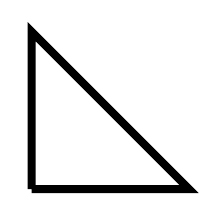
\begin{tikzpicture}%
\draw[line width=1mm](0,0) -- (0,2) -- (2,0)  -- (0,0);
\end{tikzpicture}%  
}\xspace%
}%

\newcommand{\smallltri}{%
\,\resizebox{!}{0.15\baselineskip}{%
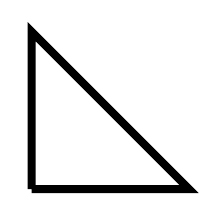
\begin{tikzpicture}%
\draw[line width=1mm](0,0) -- (0,2) -- (2,0)  -- (0,0);
\end{tikzpicture}%  
}\xspace%
}%

\title{Transport map accelerated-PAIS, and application to inverse problems arising from
  multiscale stochastic reaction networks}
\author{Simon Cotter, Yannis Kevrekidis, Paul Russell}
\begin{document}
\maketitle
\begin{abstract}
In many applications, inverse problems arise where where there are
complex correlations between the different parameters which we wish to
infer from data. The correlations often manifest themselves as lower
dimensional manifolds on which the likelihood function is
invariant, or varies very little. This can be due to trying to infer
unobservable parameters, or due to sloppiness in the model which is
being used to describe the data. In such a situation, standard
sampling methods for characterising the posterior distribution which
do not incorporate information about this structure will be highly
inefficient. Moreover, most methods are inherently serial in nature,
and as such are not expoiting the parallelised  nature of modern
computer infrastructure. In this paper, we seek to develop a method to
tackle this problem, using optimal transport maps to simplify
posterior distributions which are concentrated on lower dimensional
manifolds.

We demonstrate the approach by considering inverse problems arising
from partially observed stochastic reaction networks. In particular,
we consider systems which exhibit multiscale behaviour, but for which
only the slow variables in the system are observable. We demonstrate
that certain multiscale approximations lead to more consistent
approximations of the posterior than others.
\end{abstract}


\section{Introduction}
%Topics to cover: parallel MCMC, pMC, PAIS
%Transport maps, transport map MCMC
%Stochastic reaction networks
%Multiscale approximations, QSSA/QEA, CMA

In Section \ref{sec:map} we show how an appropriate transport map can
be constructed from importance samples which maps the posterior close
to a reference Gaussian measure. In Section \ref{sec:TPAIS} we show
how such a map can be incorporated into a sophisticated parallel MCMC
infrastructure in order to accelerate mixing. In Section
\ref{sec:conv} we seek to show the advantages of this approach through
the analysis of test problems. In Section
\ref{sec:multi} we consider how likelihoods can be approximated using
 multiscale methodologies in order to carry out inference for
multiscale and/or partially observed stochastic reaction networks. In
Section \ref{sec:num} we present some numerical examples, which serve
to demonstrate the increased efficiency of the described sampling
methodologies, as well as investigating the posterior approximations
discussed in the previous section. We conclude with a discussion in
Section \ref{sec:conc}.

\section{Construction of transport maps in importance sampling} \label{sec:map}
%Follow the other papers, show adaptation(s)

In~\cite{el2012bayesian} the transport map was introduced to provide a transformation from the prior
distribution to the posterior distribution, the idea being that one could draw a moderately sized
sample from the prior distribution and use this sample to approximate a map onto the target space.
Once this map was known to the desired accuracy a larger sample from the prior could be used to
investigate the posterior distribution. This
methodology was adapted in~\cite{parno2014transport} to form a new proposal method for MH
algorithms. In this case, rather than transforming a sample from the prior into a sample from the target
distribution, the map transforms a sample from the posterior onto a reference space.
The reference density is chosen to allow efficient proposals using a simple proposal
distribution such as a Gaussian centred at the previous state. Proposed states can then be mapped back into a sample from the posterior by applying the inverse of the transport map.

Proposing new states in this way allows us to make large steps around complex probability distributions.
It is also feasible in this framework to assume that the reference density is close enough to a standard Gaussian that we can efficiently propose moves using a proposal distribution which is independent of the current state, e.g. choose $q(\theta) = \mathcal{N}(0,I_n)$.

In this Section we outline the methodology in
\cite{parno2014transport} for approximately coupling the target,
$\mu_{\theta}$, with the reference distribution, $\mu_r$, and
show how the map can be constructed using a weighted sample
and hence how we can incorporate the map into importance sampling schemes.

\begin{dfn}[(Exact) Transport Map $T$]
	A transport map $T$ is a function $T\colon
        \mathcal{X}\rightarrow\mathbb{R}^d$ such that the {\it
          pullback} of the reference measure with density $\phi(\cdot)$,
	\begin{equation}\label{eq:pullback}
		\tilde{\pi}(\theta) = \phi(T(\theta))|J_T(\theta)|,
	\end{equation}
	is equal to the target density $\pi(\theta)$ for all $\theta \in \mathcal{X}$. The pullback is defined in terms of the determinant of the Jacobian of $T$,
	\[
		|J_T(\theta)| = \text{det}\begin{bmatrix} \partial_{\theta_1} T_1(\theta) & \dots & \partial_{\theta_d} T_1(\theta) \\ \vdots & \ddots & \vdots \\ \partial_{\theta_1} T_d(\theta) & \dots & \partial_{\theta_d} T_d(\theta) \end{bmatrix}.
	\]
\end{dfn}

% In the case that we have an invertible map,
% $T\in\mathcal{T}$ where $\mathcal{T}$ is the space of all invertible
% maps, we are able to draw a sample from $\pi_r = \phi$, the density of
% the reference distribution, which could be picked to be the
% standardised Gaussian distribution for example, and map these samples back
% onto target space using $T^{-1}$. These proposed samples are then distributed according to the target distribution.

\begin{dfn}[Target and Reference Space]
	The transport map pushes a particle from a {\it target space} $\mathcal{X}$, that is a subset of $\mathbb{R}^d$ equipped with a target measure $\mu_{\theta}$, onto a {\it reference space}, $R$, again a subset of $\mathbb{R}^d$ equipped with the reference measure $\mu_r$.
\end{dfn}

Armed with such a map, independent samples can be made of the target
measure, using the pullback of the reference density $\phi$ through $T^{-1}$.
Clearly the pullback only exists when $T$ is monotonic, i.e. has a positive definite Jacobian, and has continuous first derivatives.
Not all maps satisfy these conditions, so we define a smaller space of
maps, $\mathcal{T}^\uparrow \subset \mathcal{T}$ which contains all
feasible maps. This space does not necessarily contain an exact
coupling between target and reference space, and so we are motivated to formulate an optimisation problem to find the map $\tilde{T}
\in \mathcal{T}^\uparrow$ which most closely maps the target density
to the reference density.

% We attempt to find the deterministic coupling of two continuous
% probability distributions, $(\mu_\theta, \hat{\mu_r})$, such that
% $\hat{\mu_r} = T\mu_\theta$ where the distance between $\mu_r$ (the
% desired reference measure) and $\hat{\mu_r}$ (the achieved reference
% measure) is minimised, for $T \in \mathcal{T}^\uparrow$. As in
% \cite{parno2014transport} we aim to minimise the Kullback-Liebler (KL)
% divergence between the density of $\mu_{\theta}$ and the pullback of
% the density of $\mu_{r}$, i.e. the distance between $\pi(\theta)$ and
% $\tilde{\pi}(\theta)$. For two absolutely continuous measures with
% densities $\pi_1$ and $\pi_2$ respectively, the KL
% divergence is given by
% \[D_\text{KL}(\pi_1\|\pi_2) = 
% 		\mathbb{E}_{\pi_1}\left[\log\left(\frac{\pi_1(\theta)}{\pi_2(\theta)}\right)\right].\]
% The KL divergence is not itself a norm, since
% it is not symmetric, i.e. $D_\text{KL}(\pi_1\|\pi_2) \neq
% D_\text{KL}(\pi_2\|\pi_1)$ in general. However, it is still a useful
% measure of the similarity of two probability distributions, not least since the
% square root of the KL-divergence is an upperbound to the Hellinger
% distance metric.

As in previous work in \cite{parno2014transport}, we can ensure
invertibility if we restrict the map to be lower triangular, i.e. $\tilde{T} \in \mathcal{T}^{\ltri}\subset\mathcal{T}^\uparrow$. This lower triangular map has the form,
\[
	T(\theta_1, \dots, \theta_n) = \begin{bmatrix} T_1(\theta_1) \\ T_2(\theta_1, \theta_2) \\ \vdots \\
		T_n(\theta_1, \dots, \theta_n) \end{bmatrix},
\]
where $T_i\colon \mathbb{R}^i \to \mathbb{R}$. % We assume that the target and reference probability densities are absolutely continuous on
% $\mathbb{R}^d$. Under this formulation, with appropriate
% regularisation (which will be detailed later), we are guaranteed a unique invertible map $\tilde{T}$ with the property that
% \[
% 	\tilde{T}\mu_{\theta} \approx \mu_r.
% \]
% % Relaxing the equality constraint to finding the approximate map
% % $\tilde{T} \in \mathcal{T}^{\ltri}$ which minimises $C(T)$, gives us a
% % practical route to finding a good candidate map.

\subsection{The optimisation problem}
Our aim is now to find the lower triangular map $\tilde{T} \in
\mathcal{T}^{\ltri}$ such that the difference between target
density and the pullback of the reference density is minimised. As in
\cite{parno2014transport}, we choose the cost function
to be the Kullback-Leibler (KL) divergence between the posterior density and the pullback density,
\[
	D_\text{KL}(\pi\|\tilde{\pi}) =
		\mathbb{E}_\pi\left[\log\left(\frac{\pi(\theta)}{\tilde{\pi}(\theta)}\right)\right].
\]
This divergence results in some nice properties which we will explore in the following derivation. The KL divergence is not a true metric since it is not symmetric, however it is commonly used to measure the distance between probability distributions due to it's relatively simple form, and because it provides a bound for the square of the Hellinger distance by Pinsker's inequality~\cite{pinsker1960information},
\[
	D_{KL}(p\|q) \geq D_H^2(p,q),
\]
which is a true metric between probability distributions $p$ and $q$.
Given the form of the pullback in Equation~\eqref{eq:pullback}, now taken through an approximate map $\tilde{T}$, the divergence becomes
\[
	D_\text{KL}(\pi\|\tilde{\pi}) = \mathbb{E}_\pi\left[\log\pi(\theta) - \log\pi_r(\tilde{T}(\theta)) -
		\log\left|J_{\tilde{T}}(\theta)\right|\right].
\]
We note the posterior density is independent of $\tilde{T}$, and so it is not necessary for us to compute it when optimising this cost function. This expression is a complicated integral with respect to the target distribution, for which the normalisation constant is unknown. However this is exactly the scenario for which we would turn to MCMC methods for a solution.

To find the best coupling, $\tilde{T} \in \mathcal{T}^{\ltri}$, we solve the optimisation problem,
\[
	\tilde{T} = \arg\min_{T \in \mathcal{T}^{\smallltri}} \mathbb{E}_\pi\left[-\log\pi_r(T(\theta)) -
		\log\left|J_T(\theta)\right|\right]
\]
which has a unique solution since the cost function is convex. We also include a regularisation term, which is required for reasons which will become clear later. The optimisation problem now takes the form
\begin{equation}\label{eq:gen_map_optim}
	\tilde{T} = \arg\min_{T\in\mathcal{T}^{\smallltri}} \left[
		 \mathbb{E}_\pi\left[-\log\pi_r(T(\theta)) -
		\log\left|J_T(\theta)\right|\right] + \beta\mathbb{E}(T(\theta)- \theta)^2 \right].
\end{equation}
The parameter $\beta>0$ does not need to be tuned, as experimentation has shown that the choice
$\beta=1$ is sufficient for most problems. This expectation can be
approximated by using an MCMC approximation. The form of the penalisation term promotes maps which are
closer to the identity, and so prevents overfitting when the quality
or size of the current sample from the posterior is not sufficient.

\subsection{The structure of the map}

Before we continue with the derivation of the optimisation problem, we consider the structure
of the map in more detail. The lower triangular structure of the map not only guarantees monotonicity, it also allows for efficient calculation of the pullback density, as well as the inverse of the map, $\tilde{T}^{-1}$. The Jacobian of $\tilde{T}$ is a lower triangular matrix,
\[
	J_T(\theta) = \begin{bmatrix}
		\partial_{\theta_1} \tilde{T}_1(\theta) & \dots & \partial_{\theta_d} \tilde{T}_1(\theta)\\
		\vdots & \ddots & \vdots \\
		\partial_{\theta_1} \tilde{T}_d(\theta) & \dots & \partial_{\theta_d} \tilde{T}_d(\theta)
	\end{bmatrix} = \begin{bmatrix}
		\partial_{\theta_1} \tilde{T}_1(\theta) & \dots & 0\\
		\vdots & \ddots & \vdots \\
		\partial_{\theta_1} \tilde{T}_d(\theta) & \dots & \partial_{\theta_d} \tilde{T}_d(\theta)
	\end{bmatrix}
\]
since $\partial_{\theta_n} \tilde{T}_k(\theta) = 0$ for all $n > k$. This lower triangular structure means that the determinant of the Jacobian is a product of the diagonal elements which, when we take logs, becomes
\begin{equation}\label{eqn:separable_jacobian}
	\log\left|J_{\tilde{T}}(\theta)\right| = \sum\limits_{i=1}^d \! \log \partial_{\theta_i} \tilde{T}_i(\theta),
\end{equation}
where we note that this term is separable in terms of the dimension $i$.

Inverting $\tilde{T}$ at a point $r$ is simplified by the lower triangular structure of the map. The map component $\tilde{T}_1(\theta)$ is a univariate polynomial in $\theta_1$, so we can find the inverse of this function by solving the equation $T_1(\theta_1) = r_1$. This inversion tells us the value of $\theta_1$, which means the next component is again a univariate polynomial, $T_2(\theta_2; \theta_1)=r_2$. We can then perform $d$ root finding problems instead of a full $d$ dimensional non-linear solve.

We require that the first derivatives of the map are continuous, which is easy to enforce by the choice of basis functions. Here we assume that the map will be built from a family of orthogonal polynomials, $\mathcal{P}(\theta)$, not necessarily orthogonal with respect to the target distribution. Each component of the map is defined as a multivariate polynomial expansion,
\begin{equation}\label{eq:map_defn}
	\tilde{T}_i(\theta; \gamma_i) = \sum\limits_{\mathbf{j}\in\mathcal{J}_i} \!
\gamma_{i,\mathbf{j}}\psi_\mathbf{j}(\theta).
\end{equation}
The parameter $\gamma_i \in \mathbb{R}^{M_i}$ is a vector of coefficients. Each component of $\gamma_i$ corresponds to a basis function
$\psi_\mathbf{j}$, indexed by the multi-index $\mathbf{j} \in \mathbb{N}_0^d$. These multi-indices are elements of the multi-index set $\mathcal{J}_i$. A multi-index defines a product of univariate polynomials in $\theta_k$,
\[
	\psi_\mathbf{j}(\theta) = \prod\limits_{k=1}^i \! \varphi_{j_k}(\theta_k), \quad \text{for} \quad \mathbf{j} \in \mathcal{J}_i,
\]
and where $\varphi_{j_k}(\theta_k) \in \mathcal{P}(\theta_k)$. Since $\tilde{T}$ is lower triangular, a multi-index $\mathbf{j}\in\mathcal{J}_i$ only contains entries for univariate polynomials in $\theta_k$ for $k\leq i$.

The cardinalities of the multi-index sets, $M_i = \text{card}(\mathcal{J}_i)$, give the number of unknowns in our
optimisation problem, and so we would like to keep this number as small as possible. One option is
to use polynomials of total order $p$,
\[
	\mathcal{J}_i^\text{TO} = \left\{\mathbf{j}:\|\mathbf{j}\|_1 \leq p, j_k = 0\ \forall k > i\right\},
\]
which is optimal in terms of the amount of information captured by the map about the target. The cardinality of $\mathcal{J}_i^\text{TO}$ is $M_i = \binom{i+p}{p}$ which increases rapidly in $d$ and $p$, where $i = 1, \dots, d$. Smaller optimisation problems can be produced by constructing subsets of $\mathcal{J}_i^\text{TO}$. These index sets are discussed
in~\cite{parno2014transport}. Increased information with a slower increase in the number of map parameters can be achieved with the composition of maps discussed in~\cite{parno2015transport}. Here we stick with polynomials of total order $p$ since we work with low dimensional problems with the PAIS algorithm.


\subsection{Implementation of the optimisation problem}\label{sec:transport_implementation}

We now discuss how we can evaluate the cost function in
Equation~\eqref{eq:gen_map_optim}. In \cite{parno2014transport}, this
expectation is approximated using an MCMC estimator, such that
\begin{align}
	C(T) &= \mathbb{E}_\pi\left[ -\log\pi_r(T(\theta)) - \log|J_T(\theta)|\right] +
			\beta\mathbb{E}(T(\theta)-\theta)^2 \notag \\
		&\approx \frac{1}{K}\sum\limits_{i=1}^d \! \sum\limits_{k=1}^K \left[-\log\pi_r(T_i(\theta^{(k)})) -
			\log\left|\frac{\partial T_i}{\partial \theta_i}(\theta^{(k)})\right| + \beta(T_i(\theta^{(k)})-\theta^{(k)})^2\right]. 
\end{align}
Here we diverge from previous work, as we aim to build a map from
samples from an importance sampling scheme. Such samples no longer
carry equal weight, and as such the Monte Carlo estimator becomes
\begin{equation}\label{eqn:TM_full_cost}
	C(T) = \frac{1}{\bar{w}}\sum\limits_{i=1}^d \! \sum\limits_{k=1}^K
		w_k \left[-\log\pi_r(T_i(\theta^{(k)})) -
			\log\left|\frac{\partial T_i}{\partial \theta_i}(\theta^{(k)})\right| + \beta(T_i(\theta^{(k)})-\theta^{(k)})^2\right],
\end{equation}
where $w_k$ are the weights associated with each sample $\theta^{(k)}$, and $\bar{w}$ is the sum of
all these weights. Optimisation of this cost function results in a map from $\pi$ to some reference density $\pi_r$. By choosing the reference density to be a Gaussian density, we can simplify this expression greatly. Substitution of the Gaussian density into Equation~\eqref{eqn:TM_full_cost} leads to
\begin{equation}\label{eqn:TPAIS_objective}
	C(T) = \frac{1}{\bar{w}}\sum\limits_{i=1}^d \! \sum\limits_{k=1}^K
		w_k\left[\frac{1}{2}T_i^2(\theta^{(k)}) - \log\frac{\partial
		T_i}{\partial\theta_i}(\theta^{(k)}) + \beta(T_i(\theta^{(k)})-\theta^{(k)})^2\right],
\end{equation}

Note that since we assume that the map is monotonic, the derivatives of each component are
positive and so this functional is always finite. In practice it is infeasible to enforce this condition across the whole parameter space. We instead enforce this condition by ensuring that the derivatives are positive at each sample point. This means that when we sample away from these support points while in reference space, it is possible to enter a region of space where the map is not monotonic.

We now return to the structure of the map components given in Equation~\eqref{eq:map_defn}. Since the basis functions are
fixed, the optimisation problem in \eqref{eq:gen_map_optim} is really over the map components $\bar{\gamma} = (\gamma_1, \dots,
\gamma_d)$ where $\gamma_i \in \mathbb{R}^{M_i}$. Note that $C(T)$ is the sum of $d$ expectations, and these expectations each only concern one dimension. Therefore we can rewrite \eqref{eq:gen_map_optim} as $d$ separable optimisation problems.
\begin{align}\label{eq:gamma_map_optim}
	&\arg\min_{\gamma_i\in\mathbb{R}^{M_i}} \frac{1}{\bar{w}}\sum\limits_{k=1}^K
		w_k \left[\frac{1}{2}T_i^2(\theta^{(k)}; \gamma_i) - \log\frac{\partial T_i}{\partial\theta_i}(\theta^{(k)}; \gamma_i) + \beta(T_i(\theta^{(k)};
		\gamma_i)-\theta^{(k)})^2\right], \\
	&\text{subject to} \quad \frac{\partial T_i}{\partial\theta_i}(\theta^{(k)};
		\gamma_i) > 0 \ \text{for all}\ k=1,\dots,K,\ i=1,\dots,d.
		\notag
\end{align}
The sum in Equation~\eqref{eq:map_defn} is an inner
product between the vector of map coefficients, and the evaluations of the basis function at a
particular $\theta^{(k)}$. If we organise our basis evaluations into two matrices,
\[
	(F_i)_{k,\mathbf{j}} = \psi_\mathbf{j}(\theta^{(k)}), \quad \text{and} \quad (G_i)_{k,\mathbf{j}} =
\frac{\partial\psi_\mathbf{j}}{\partial\theta_i}(\theta^{(k)}),
\]
for all $\mathbf{j}
\in \mathcal{J}_i^\text{TO}$, and $k = 1,\dots,K$, then we have that
\[
	T_i(\theta^{(k)}) = (F_i)_{k\cdot}\gamma_i \quad \text{and} \quad \frac{\partial T_i}{\partial \theta_i}(\theta^{(k)}; \gamma_i) = (G_i)_{k\cdot}\gamma_i,
\]
so \eqref{eq:gamma_map_optim} becomes
\begin{align}\label{eq:blas_map_optim}
	&\arg\min_{\gamma_i\in\mathbb{R}^{M_i}}
          \frac{1}{2}(F_i\gamma_i)^\top W (F_i\gamma_i) -
		{\bf w}^\top\log(G_i\gamma_i) + \frac{\beta}{\bar{w}}\sum\limits_{k=1}^K \!
		w_k(F_i\gamma_i-\theta^{(k)})^\top(F_i\gamma_i-\theta^{(k)}), \\
	&\text{subject to} \quad G_i\gamma_i > 0. \notag
\end{align}
In this expression, the vector ${\bf w} = [w_1, w_2, \ldots,
w_K]^\top$ is the vector of the weights, $W$ is the diagonal matrix $W
= \text{diag}(w)$ and $\log(G_i\gamma_i)$ is to be
evaluated element-wise. As more importance samples are made, new rows can be appended to the
$F_i$ and $G_i$ matrices, and $F_i^\top W F_i$ can be efficiently updated via the addition of rank-1 matrices.

The regularisation term in Equation~\eqref{eq:blas_map_optim} can be approximated using Parseval's identity,
\[
	\frac{1}{\bar{w}}\sum\limits_{k=1}^K \! w_k
        (F_i\gamma_i-\theta^{(k)})^\top(F_i\gamma_i-\theta^{(k)})
        \xrightarrow[K \to \infty]{}
		\int_{\mathbb{R}^n} |T(\theta)-\theta|^2 \text{d}\mu_\theta =
		\sum\limits_{\mathbf{j}\in\mathcal{J}_i^\text{TO}} (\gamma_{i,\mathbf{j}}-\iota_\mathbf{j})^2,
\]
where $\iota$ is the vector of coefficients for the identity map. This is of course only true when
the polynomial family $\mathcal{P}(\theta)$ is chosen to be orthonormal with respect to $\mu_\theta$; however this
approximation prevents the map from collapsing onto a Dirac when the expectation is badly approximated by a small number of samples.% If we do not normalise the MC estimator by $K$, we can allow this regularisation term to be dominated by the rest of the cost function as $K$ increases.

These simplifications result in the efficiently implementable, regularised optimisation problem for
computing the map coefficients, 
\begin{align}\label{eq:weighted_map_optim}
	&\arg\min_{\gamma_i\in\mathbb{R}^{M_i}} \frac{1}{2\bar{w}}\gamma_i^\top F_i^\top WF_i\gamma_i -
		\frac{w^\top}{\bar{w}}\log(G_i\gamma_i) + \beta\|\gamma_i-\iota\|^2, \\
	&\text{subject to} \quad G_i\gamma_i > 0, \notag
\end{align}
%where additionally we have introduced a factor of $\frac{1}{K}$ to the
%regularisation term to prevent over-smoothing as the number of samples increases.
This optimisation problem can be efficiently solved using Newton iterations. It is suggested
in~\cite{parno2014transport} that this method usually converges in around 10-15 iterations, and we
have seen no evidence that this is not a reasonable estimate. When calculating the map several times
during a Monte Carlo run, using previous guesses of the optimal map to seed the Newton algorithm
results in much faster convergence, usually taking only a couple of iterations to satisfy the stopping
criteria.

The Hessian takes the
form
\begin{equation}\label{eqn:TPAIS_hessian}
	HC_i(\gamma_i) = \frac{1}{\bar{w}}\left[F_i^\top WF_i + G_i^\top
		W\text{diag}([G_i\gamma_i]^{-2})G_i\right] + \beta I,
\end{equation}
where $[G_i\gamma_i]^{-2}$ is to be taken element-wise, and $I$ is the $M_i\times M_i$
identity matrix. The first derivative of $C_i(T)$ is
\[
	\nabla C_i(\gamma_i) = \frac{1}{\bar{w}}\left[F_i^\top WF_i\gamma_i - G_i^\top
		W[G_i\gamma_i]^{-1}\right] + \beta(\gamma_i - \iota),
\]
again $[G_i\gamma_i]^{-1}$ is taken element-wise.



\section[Transport map MCMC]{Transport map usage in PAIS
  and other PMC algorithms}\label{sec:TPAIS}

Given importance samples from the target distribution, we have demonstrated how to construct an approximate transport map from the
target measure to a reference measure. We now consider how to
implement an importance sampling-based MCMC algorithm which uses
these maps to propose new states. In \cite{parno2014transport} it was
shown how approximate transport maps can be used to accelerate
Metropolis-Hastings methods, with the map being periodically updated
with the samples produced from the target measure. Convergence of this
adaptation is shown in~\cite{parno2014transport}. In this Section, we
will show how similarly, these maps can be used to construct highly
efficient importance sampling schemes.

In particular, we will show how we can use the transport map derived in Equation~\eqref{eq:weighted_map_optim} to
design a proposal scheme for the PAIS algorithm. In this case we have a choice in how to proceed; we
propose new samples on reference space and resample on target space, or we both propose and resample on reference space, mapping onto target space to output the samples. The first option allows us to reuse much of the framework
from the standard PAIS algorithm and in the numerics later we see that this performs better than
both the Transport MH algorithm, and the standard PAIS algorithm. The second option requires some
restructuring but results in improved performance from the resampler.

\begin{table}
\begin{algorithm}[H]
\DontPrintSemicolon
\BlankLine
Initialise state $\theta^{(1)}_i = \theta_0$, \quad $i = 1,\dots,M$.\;
Initialise map $\bar{\gamma}^{(1)} = \iota$.\;
\For{$k \leftarrow 1, \dots, L-1$}{
	Compute $r_i = \tilde{T}(\theta^{(k)}_i; \bar{\gamma}^{(k)})$, \quad $i = 1,\dots,M$.\;
	Sample $r'_i \sim q_r(\cdot; r_i)$.\;
	Invert $\hat{\theta}_i^{(k)} = \tilde{T}^{-1}(r'_i; \bar{\gamma}^{(k)})$.\;
	Calculate:
	\[
		w_i^{(k)} = \frac{\pi(\hat{\theta}_i^{(k)})}{\left(\sum_{j=1}^M \! q_r(r_i'; r_j)\right)|J_{\tilde{T}}(\hat{\theta}_i^{(k)};\bar{\gamma}^{(k)})|}.
	\]

	Resample $\theta^{(k+1)} \leftarrow \|w^{(k)}\|^{-1}\sum\limits_{j=1}^M \! w_j^{(k)}\delta_{\hat{\theta}^{(k)}_j}(\cdot)$.\;

	\eIf{$k\ \text{mod}\ K_U = 0$ and $k < K_\text{stop}$}{
		\For{$i \leftarrow 1, \dots, n$}{
			Solve \eqref{eq:weighted_map_optim} with $\{(w^{(1)},\hat{\theta}^{(1)}), \dots, (w^{(k+1)},\hat{\theta}^{(k+1)})\}$
				and update $\gamma_i^{(k+1)}$.\;
		}
	}{
		$\bar{\gamma}^{(k+1)} = \bar{\gamma}^{(k)}$.\;
	}
}
\caption{PAIS algorithm with adaptive transport map. Option 1.\label{alg:TransportPAIS1}}
\end{algorithm}
\end{table}

The first option is given in Algorithm~\ref{alg:TransportPAIS1}. We
denote the ensembles of states in target space $\theta^{(k)} =
\{\theta^{(k)}_1,\dots,\theta^{(k)}_M\}$, and the states in the
reference space, $r = \{r_1,\dots,r_M\}$, where $M$ is the ensemble
size. Similarly, the proposal states are denoted $r' =
\{r'_1,\dots,r'_M\}$ and $(w^{(k)}, \hat{\theta}^{(k)}) =
\{(w^{(k)}_1, \hat{\theta}^{(k)}_1),\dots,(w^{(k)}_M,
\hat{\theta}^{(k)}_M)\}$, where these pairs are the states which
together form our sample from the target distribution. As in the standard version of the PAIS algorithm we use the deterministic mixture weights.

\begin{table}
\begin{algorithm}[H]
\DontPrintSemicolon
\BlankLine
Initialise state $\theta^{(1)}_i = \theta_0$, \quad $i = 1,\dots,M$.\;
Initialise map $\bar{\gamma}^{(1)} = \iota$.\;
\For{$k \leftarrow 1, \dots, N-1$}{
	Compute $r_i = \tilde{T}(\theta^{(k)}_i; \bar{\gamma}^{(k)})$, \quad $i = 1,\dots,M$.\;
	Sample $r'_i \sim q_r(\cdot; r_i)$.\;
	Invert $\hat{\theta}_i^{(k)} = \tilde{T}^{-1}(r'_i; \bar{\gamma}^{(k)})$.\;
	Calculate:
	\[
		w_i^{(k)} = \frac{\pi(\hat{\theta}_i^{(k)})}{\left(\sum_{j=1}^M \! q_r(r_i'; r_j)\right)|J_{\tilde{T}}(\hat{\theta}_i^{(k)};\bar{\gamma}^{(k)})|}.
	\]

	Resample $r^* \leftarrow \|w^{(k)}\|^{-1}\sum\limits_{j=1}^M \! w_j^{(k)}\delta_{r'_j}(\cdot)$.\label{algline:TPAIS_resample}\;
	Invert $\theta^{(k+1)}_i = \tilde{T}^{-1}(r^*_i)$.\;
	\eIf{$k\ \text{mod}\ K_U = 0$ and $k < K_\text{stop}$}{
		\For{$i \leftarrow 1, \dots, n$}{
			Solve \eqref{eq:weighted_map_optim} with $\{(w^{(1)},\hat{\theta}^{(1)}), \dots, (w^{(k+1)},\hat{\theta}^{(k+1)})\}$
				and update $\gamma_i^{(k+1)}$.\;
		}
	}{
		$\bar{\gamma}^{(k+1)} = \bar{\gamma}^{(k)}$.\;
	}
}
\caption{PAIS algorithm with adaptive transport map. Option 2.\label{alg:TransportPAIS2}}
\end{algorithm}
\end{table}

The second option, Algorithm~\ref{alg:TransportPAIS2}, is similar to
the first except on Line~\ref{algline:TPAIS_resample} where rather
than resampling in target space we resample in reference space. In
reference space the dimensions are roughly uncorrelated, and the
Gaussian marginals are easy to approximate with fewer ensemble
members. This means that the resampling step will be more efficient in
moderately higher dimensions, which we discuss in Section~\ref{sec:TPAIS_higher_dim}.

\section[Convergence of transport MCMC]{Convergence of the transport proposal based MCMC algorithms}\label{sec:conv}

In this Section we study the convergence of the transport based
proposal distributions which we have described in
Section~\ref{sec:TPAIS}.
We take as a test problem the ubiquitous Rosenbrock banana-shaped
density. This target density is given by
\begin{equation}\label{eqn:R2_repeat}
	\pi(\theta) = \frac{\sqrt{10}}{\pi}\exp\left\{ -(1 - \theta_1)^2 - 10(\theta_2 - \theta_1^2)^2 \right\}.
\end{equation}
A contour plot of the target density is given in Figure~\ref{fig:R2_posterior}.
\begin{figure}
\centering
\subfigure[Marginal density function for $\theta_1$.]{\includegraphics[width=0.31\textwidth]{"images/TPAIS/R2_marginal_1"}}
\subfigure[Marginal density function for $\theta_2$.]{\includegraphics[width=0.31\textwidth]{"images/TPAIS/R2_marginal_2"}}
\subfigure[Contour plot for Rosenbrock density.]{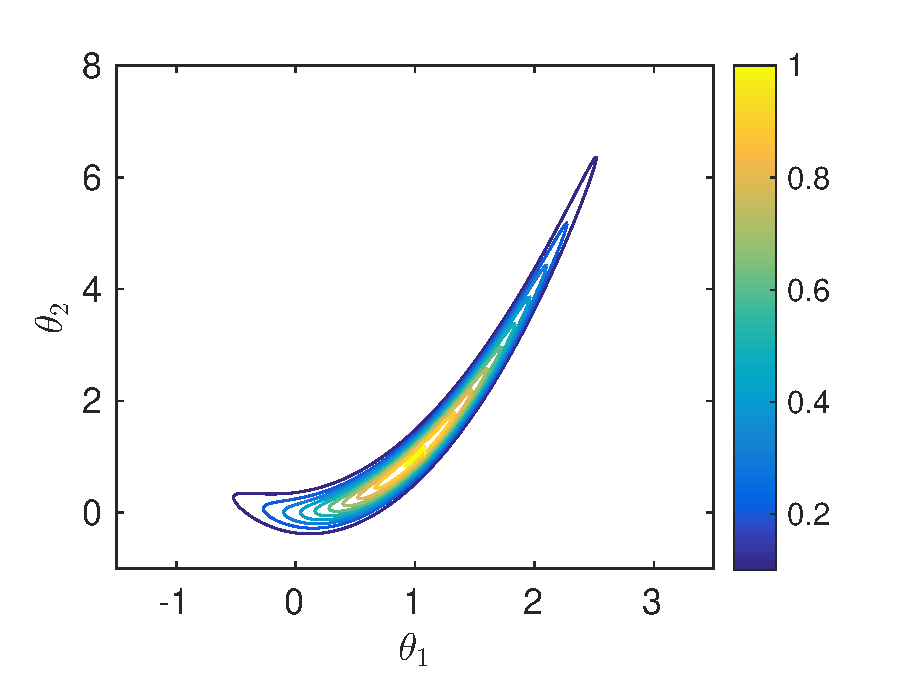
\includegraphics[width=0.31\textwidth]{images/TPAIS/R2_posterior}}
\caption{Visualisation of the Rosenbrock density as given in Equation~\eqref{eqn:R2_repeat}.}
\label{fig:R2_posterior}
\end{figure}
This problem is challenging to sample from since it has a highly peaked and curved ridge, and is often used
as a test problem in optimisation and MCMC communities.

\subsection{Implementation details}

Before looking at the performance of the MCMC algorithms, we demonstrate some properties of the transport maps we will be using in our MCMC algorithms. We draw 1 million samples from the density in \eqref{eqn:R2_repeat}, and use this sample in the framework of Section~\ref{sec:map} to build a transport map. We use this map to push forward the original sample onto the reference space, where we will be able to see how well the map has performed at converting the original sample to a standard Gaussian. We then pull the sample back on to target space using the inverse map to check that our map is invertible and well behaved.

For this example, we use an index set of total order 3 with monomial
basis functions. It is important that total order is an odd number,
since otherwise the map will not be surjective. This results in a map of the form
\[
	T(\theta_1, \theta_2) = \begin{bmatrix} T_1(\theta_1) \\ T_2(\theta_1, \theta_2) \end{bmatrix},
\]
where
\begin{align*}
		T_1(\theta_1) &= \gamma_{1,1} + \gamma_{1,2}\theta_1 + \gamma_{1,3}\theta_1^2 + \gamma_{1,4}\theta_1^3, \\
		T_2(\theta_1, \theta_2) &= \gamma_{2,1} + \gamma_{2,2}\theta_1 + \gamma_{2,3}\theta_1^2 + \gamma_{2,4}\theta_1^3
					+ \gamma_{2,5}\theta_2 + \gamma_{2,6}\theta_1\theta_2 \\
				 & \qquad \quad + \gamma_{2,7}\theta_1^2\theta_2 + \gamma_{2,8}\theta_2^2 + \gamma_{2,9}\theta_1\theta_2^2 +
					 \gamma_{2,10}\theta_2^3.
\end{align*}
Clearly even with only basis functions of total order 3, we have a large number of unknowns in our optimisation problem, $\bar{\gamma} \in \mathbb{R}^{14}$. If we were to increase the dimension of $\theta$ further we would need to reduce the number of terms we include in the expansion by, for example, removing all the ``cross'' terms. This reduces the quality of our map but since we only require an approximate map we can afford to reduce the accuracy.

\begin{figure}[htpb]
\centering
\subfigure[Original sample $\theta$ from RWMH algorithm.]{\includegraphics[width=0.31\textwidth]{"images/TPAIS/R2_transport_orig"}}\quad
\subfigure[Push forward of $\theta$ onto reference space.]{\includegraphics[width=0.31\textwidth]{"images/TPAIS/R2_transport_ref"}}\quad
\subfigure[Pull back of reference sample onto target space.]{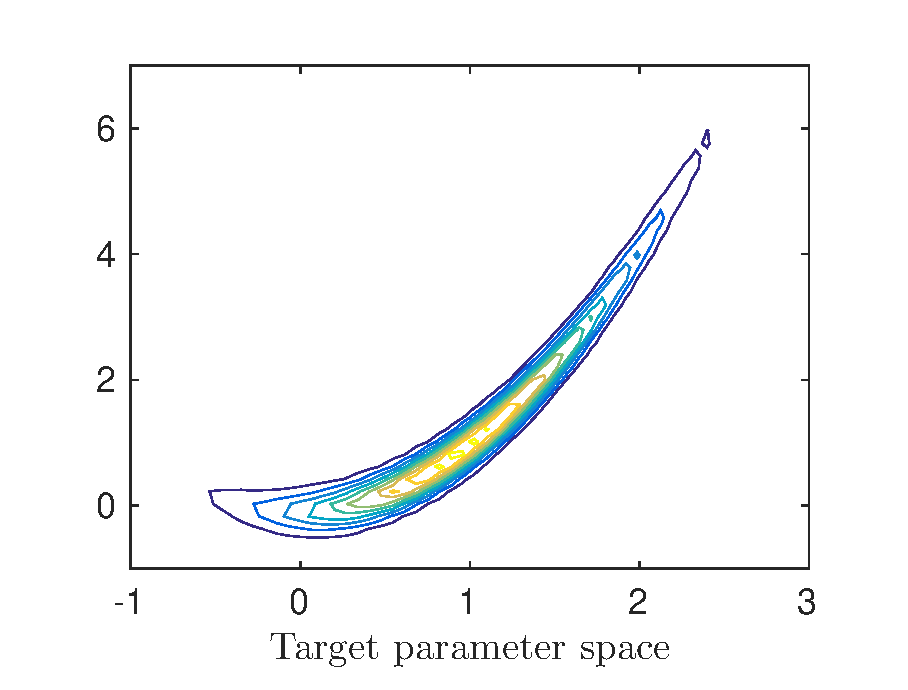
\includegraphics[width=0.31\textwidth]{images/TPAIS/R2_transport_pullback}}
\caption{Rosenbrock target density as described in Equation~\eqref{eqn:R2_repeat}.}
\label{fig:R2_transport}
\end{figure}

Figure~\ref{fig:R2_transport} shows the output of the approximate
transport map. Even though we have truncated the infinite expansion in
the monomial basis down to 4 and 10 terms in respective dimensions,
the push forward of the sample is still a unimodal distribution
centred at the origin with standard deviation 1. As you move out into
the tails of the reference density more non-Gaussian features are
clearly visible. However, overall, the push forward of the target
density does not look a challenging one to sample from, with even
relatively simple MCMC methods such as RWMH. The pullback from
reference space, in Figure~\ref{fig:R2_transport}, is an exact match
of the original sample since we have not perturbed the sample in
reference space. This inversion is well defined in the sampling
region, although not necessarily outside\cite{parno2014transport}.

\subsection[Numerical results]{Numerical results for convergence of
  transport map based algorithms on the Rosenbrock density}

We first find the optimal scaling parameters for the individual
algorithms. This is done, as in ****CITE US**** by optimising for the effective sample size in
the PAIS algorithm, and by tuning the relative $L^2$ error in the MH
algorithm. There is currently no
guidance on the best way of tuning the MH algorithm with transport map
proposals although one might expect results similar to the standard MH
results, especially if adaptation of the map is stopped after a given
point. As in the PAIS algorithm, optimising for the effective sample size might be the best option.

\begin{table}[!ht]
\centering
\begin{tabular}{lrrr}
\toprule
	Statistic \quad / \quad Algorithm & Transport M-H &
                                                            Alg. \ref{alg:TransportPAIS1} & Alg. \ref{alg:TransportPAIS2}  \\ \cmidrule(lr){1-4}
	$\delta_{L^2}$				 & 1.0e-0 & 1.1e-1 & 3.5e-1 \\
	$\delta_{\text{ESS}}$				 & - & 1.0e-1 & 5.2e-1 \\ \cmidrule(lr){1-4}
	Acc. rate							 & 0.23 & - & - \\
	ESS ratio							 & - & 0.62 & 0.71 \\
\bottomrule
\end{tabular}
\caption{Optimal scaling parameters for the transport map based algorithms applied to $R_1$.}
\label{tab:R2_opt_scaling}
\end{table}

The optimal scaling parameters are given in
Table~\ref{tab:R2_opt_scaling}. Here we see that the effective sample
size is much lower than we see in the one-dimensional examples with
the PAIS algorithms. However, in the Rosenbrock density
\eqref{eqn:R2_repeat} we are dealing with a much more complicated
correlation structure, as well as a very slowly decaying tail in
$\theta_2$. From our experiments, we have observed that the standard PAIS-RW required an ensemble size of $M=500$ to overcome the problems in this density, however the transport map transforms the tails to be more like those of a Gaussian which can be approximated well by a smaller ensemble size of $M=150$.

\begin{figure}[!ht]
\centering
\subfigure[Comparison of the two Transport PAIS options.]{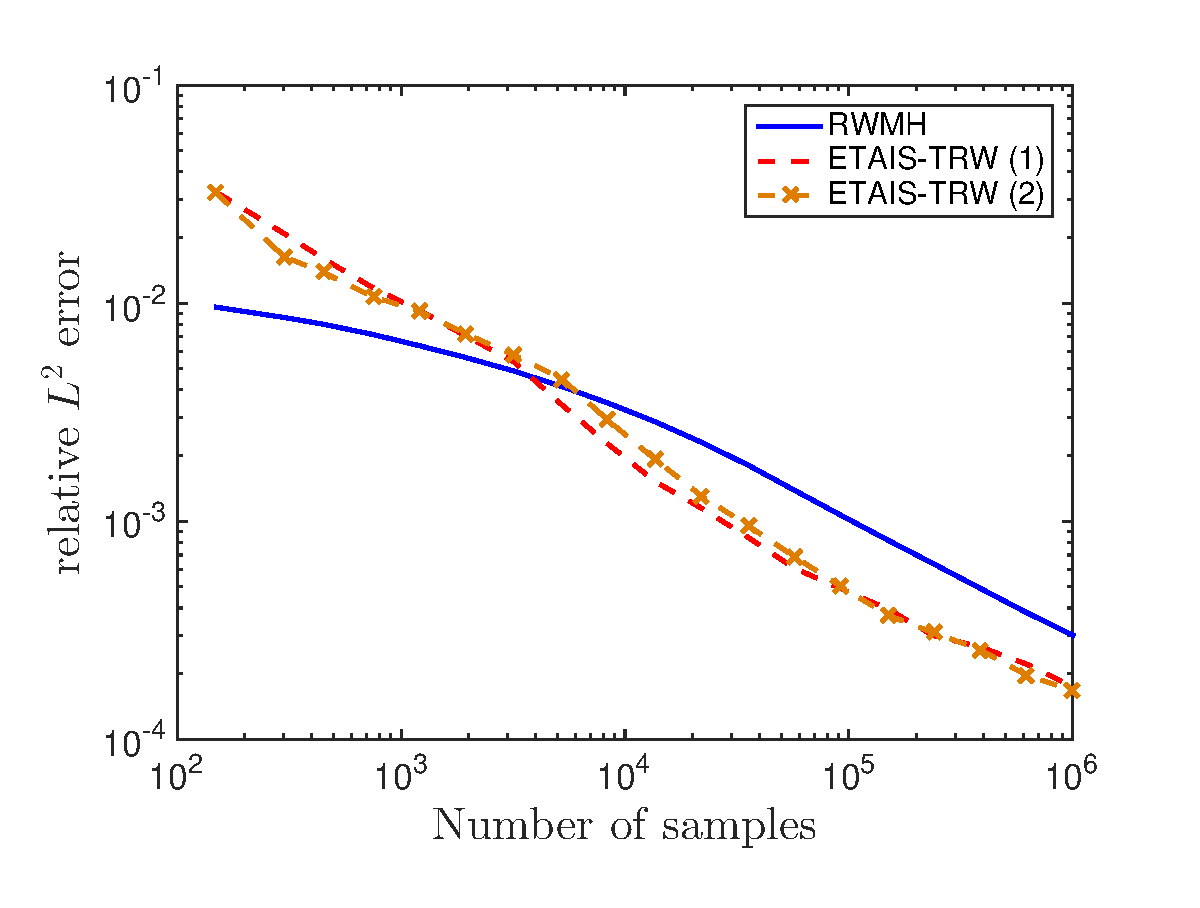
\includegraphics[width=0.45\textwidth]{images/TPAIS/R1_L2}}
\subfigure[Comparison of Transport PAIS option (2) with the standard algorithms.]{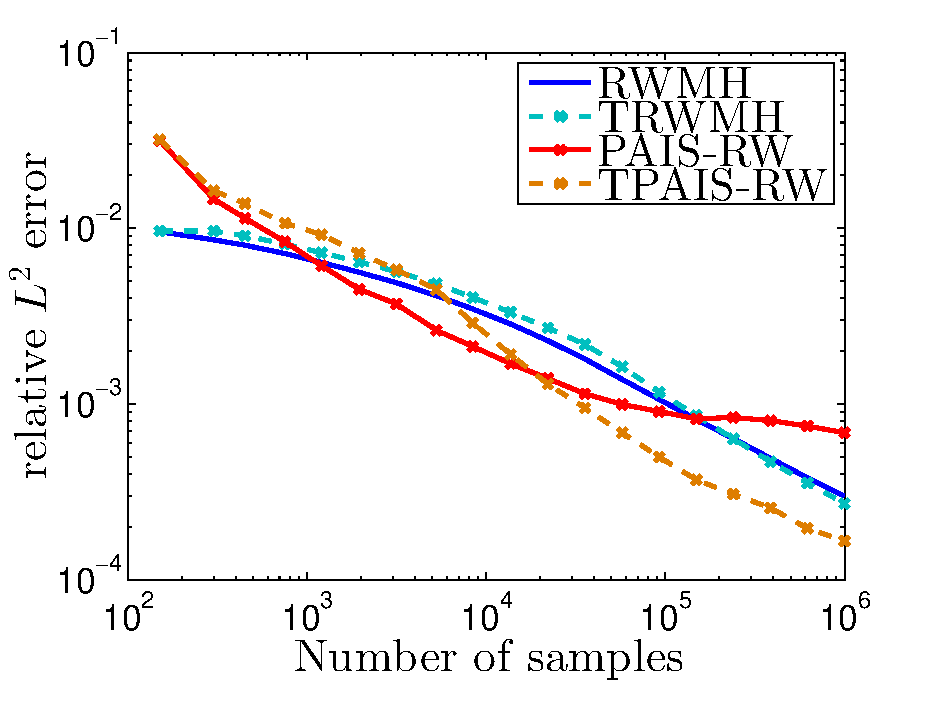
\includegraphics[width=0.45\textwidth]{images/TPAIS/R1_L2_all}}
\caption{Convergence of Algorithms Transport M-H,
  \ref{alg:TransportPAIS1}, \ref{alg:TransportPAIS2} for density \eqref{eqn:R2_repeat}. Ensemble size $M=150$, resampling performed using the AMR algorithm.}
\label{fig:R2_l2_convergence}
\end{figure}

The convergence of the three algorithms is displayed in Figure~\ref{fig:R2_l2_convergence}. Figure (a) shows that the two variations of the transport based PAIS algorithms converge with similar rates. The second version, which performs the resampling stage in reference space rather than target space, has a slightly higher ESS, and is more stable than option (1). This version also has a property that we can exploit in Section~\ref{sec:TPAIS_higher_dim}.


%\section{Transport map-accelerated Parallel Adaptive Importance
  %Sampling (TPAIS)}\label{sec:TPAIS}

\section{Multiscale Methods for Stochastic Chemical Reaction
  Networks}\label{sec:multi}
In this Section, we discuss some recent advances in multiscale methods
for stochastic reaction networks. Inverse problems arising in this
area often lead to highly correlated and complex posterior
distributions, which traditional MCMC methods can struggle to sample
from. We will then go on to solve some inverse problems related to
this in Section \ref{sec:num}.

\section{Numerical Examples}\label{sec:num}

\section{Discussion}\label{sec:conc}

\subsection{Sampling in (moderately) higher
  dimensions}\label{sec:TPAIS_higher_dim}
One major problem with importance sampling schemes is the curse of
dimensionality, which means that methods such as PAIS, and other PMC
methods, can only be used for relatively low dimensional
problems. Here, we will briefly discuss how transport maps could aid
with making moderately higher dimensional problems accessible to this
family of methods.

Algorithm~\ref{alg:TransportPAIS2} allows us to decorrelate the dimensions of our random parameter on reference space, where we then can resample and map the resulting ensemble back onto target space. Since, on reference space, the dimensions are uncorrelated, we are able to resample in each dimension separately. Resampling in a single dimension allows for optimisations in resampling code, and also means that the resampler is not affected by the curse of dimensionality.

If we can approximate the posterior well with our mixture and with the
transport map, we should not be affected by the increase in dimension
to the extent we have been with the standard PAIS-RW algorithm. In one
dimension the ETPF algorithm can be implemented very efficiently. As
described in~\cite{reich2013nonparametric}, the coupling matrix has
all non-zero entries in a staircase pattern when the state space is
ordered. We can exploit this knowledge to produce
Algorithm~\ref{alg:ETPF_1d}. Which is much faster than using the
simplex algorithm to minimise the associated cost function, and faster
than the AMR algorithm****CITE OUR OTHER PAPER****.

\begin{table}[!htpb]
\begin{algorithm}[H]
\DontPrintSemicolon
\BlankLine
Sort the states, $\{(w_i, x_i)\}_{i=1}^M$, into ascending order.\;
Normalise the weights $p_i = w_i/\|w\|_1$.\;
Set $y_i \leftarrow 0$ for all $i=1,\dots,M$.\;
Set $c \leftarrow 0$\;
\For{$i \leftarrow 1, \dots, M$}{
	Set $t \leftarrow p_i$\;
	\While{$j \leq M$ and $t > 0$}
	{
		Set $s \leftarrow \left(M^{-1}-c\right) \wedge t$\;
		Increase $y_j$ by $M\times s\times x_i$.\;
		Decrease $t$ by $s$.\;
		Increase $c$ by $s$.\;
		\If{$t>0$}
		{
			Increase $j$ by 1.\;
			Set $c \leftarrow 0$.
		}
	}
}
Return $y$.\;
\caption{ETPF algorithm in one dimension.\label{alg:ETPF_1d}}
\end{algorithm}
\end{table}


\bibliographystyle{siam}
\bibliography{bibliography}

\end{document}